%! Author = jbf
%! Date = 31.07.25

\newpage
\section{Grundlagen}
\label{sec:grundlagen}

In diesem Kapitel werden die theoretischen Grundlagen für das Entwickeln der Software,
so wie das notwendige Verständnis des Teststandes und seine Abläufe behandelt.


\subsection{Überblick über den Umrichter-Prüfstand}
\label{subsec:uberblick-uber-den-umrichter-prufstand}

In diesem Abschnitt wird der Umrichter-Teststand, von dem die zu verarbeitenden Datensätze stammen, beschrieben,
da dies für das generelle Verständnis der einzulesenden Datensatzstruktur unerlässlich ist.
Die genaue Bezeichnung des Teststandes „USTB DWT Test Bench (XCT0006-1)“ wird im Folgenden als Test-Bench oder Teststand benannt.
Diese Art Test-Bench wird im Allgemeinen für die End-of-Line-Prüfung von unterschiedlichen Umrichtern nach ihrer Herstellung genutzt,
um die Produktqualität und -funktionalität sicherzustellen. \cite*{Main_Manuel_USTB2018}

In dem hier vorliegenden Fall wird der Teststand verwendet, um die aus dem Feld kommenden Umrichter auf ihre weitere Nutzungstauglichkeit zu testen.
Die weitere Nutzungstauglichkeit wird ermittelt, indem die Messwerte mit Mittelwerten, die von mehreren fabrikneuen Umrichtern stammen, verglichen werden.
Diese Messwerte müssen sich in einem vorher definierten Toleranzbereich befinden, um weiter im Feld verwendet zu werden.

Die Umrichter werden in der gegebenen Fachliteratur zur Test-Bench als \ac{DUTs} bezeichnet.
Diese Bezeichnung kommt auch in den Berichten auf dem Teststand vor, daher hat der Autor diese Abkürzung übernommen.

%------------------------------------------------------------------------------------------------------
\subsubsection{Aufbau des Teststandes}
%------------------------------------------------------------------------------------------------------
Die Test-Bench besteht aus mehreren Komponenten, die sich im Testraum in unterschiedlichen Schaltschränken befinden.
Der Teststand besteht aus folgenden Hauptkomponenten:
Die Test-Bench besteht aus mehreren Komponenten, die sich im Testraum in unterschiedlichen Schaltschränken befinden, und der Teststand umfasst folgende Hauptkomponenten:
\begin{itemize}

\item Das Netzteil wandelt die 400-V-Netzspannung in eine isolierte Gleichspannung für den Zwischenkreis um.
Das Netzteil liefert maximal 80 kW mit 1200 V DC oder 800 V DC, welche Werte verwendet werden, kann vor Teststart bestimmt werden.
In Abbildung \ref{fig: Aufbau des Teststandes} wird das Netzteil als PSU bezeichnet, was für „Power Supply Unit“ steht.
\item Das Elektronik-Rack, auf dem die Mess- und Steuerkomponenten befestigt sind, ist ein wichtiger Bestandteil des Teststandes.
Hier befindet sich auch der (XCS2100) System-Controller, der das ganze System mit dem PC, auf dem die Test-Bench-Software läuft, via Ethernet verbindet.
In Abbildung \ref{fig: Aufbau des Teststandes} mit ER bezeichnet, für „Electronic Rack“.
\item Der Testmatrix-Schrank, in dem die Sammelschienen für den Stromanschluss und die Schützen sitzen.
In Abbildung \ref{fig: Aufbau des Teststandes} mit TM bezeichnet, für „Test Matrix cabine“.
\item Der Schrank mit dem Kühlungssystem, da die Umrichter während des Betriebes mit Wasser oder Luft gekühlt werden müssen.
In Abbildung \ref{fig: Aufbau des Teststandes} mit „Cool1“ bezeichnet.
\item Der Carrier, auf dem die Umrichter befestigt werden, ist speziell für bestimmte Umrichter konstruiert.
Dieser wird speziell für bestimmte Umrichter konstruiert.
In Abbildung \ref{fig: Aufbau des Teststandes} wird der Carrier als Carrier1 bezeichnet.

\end{itemize}

Neben den Hauptkomponenten befinden sich außerhalb des Sicherheitsbereiches, der während des Betriebes nicht betreten werden darf,
ein PC mit einer Software zum Steuern der Testeinrichtung sowie eine Betriebsanzeige und ein Notaus. \cite*{Main_Manuel_USTB2018}

\begin{figure}[h]
    \centering
    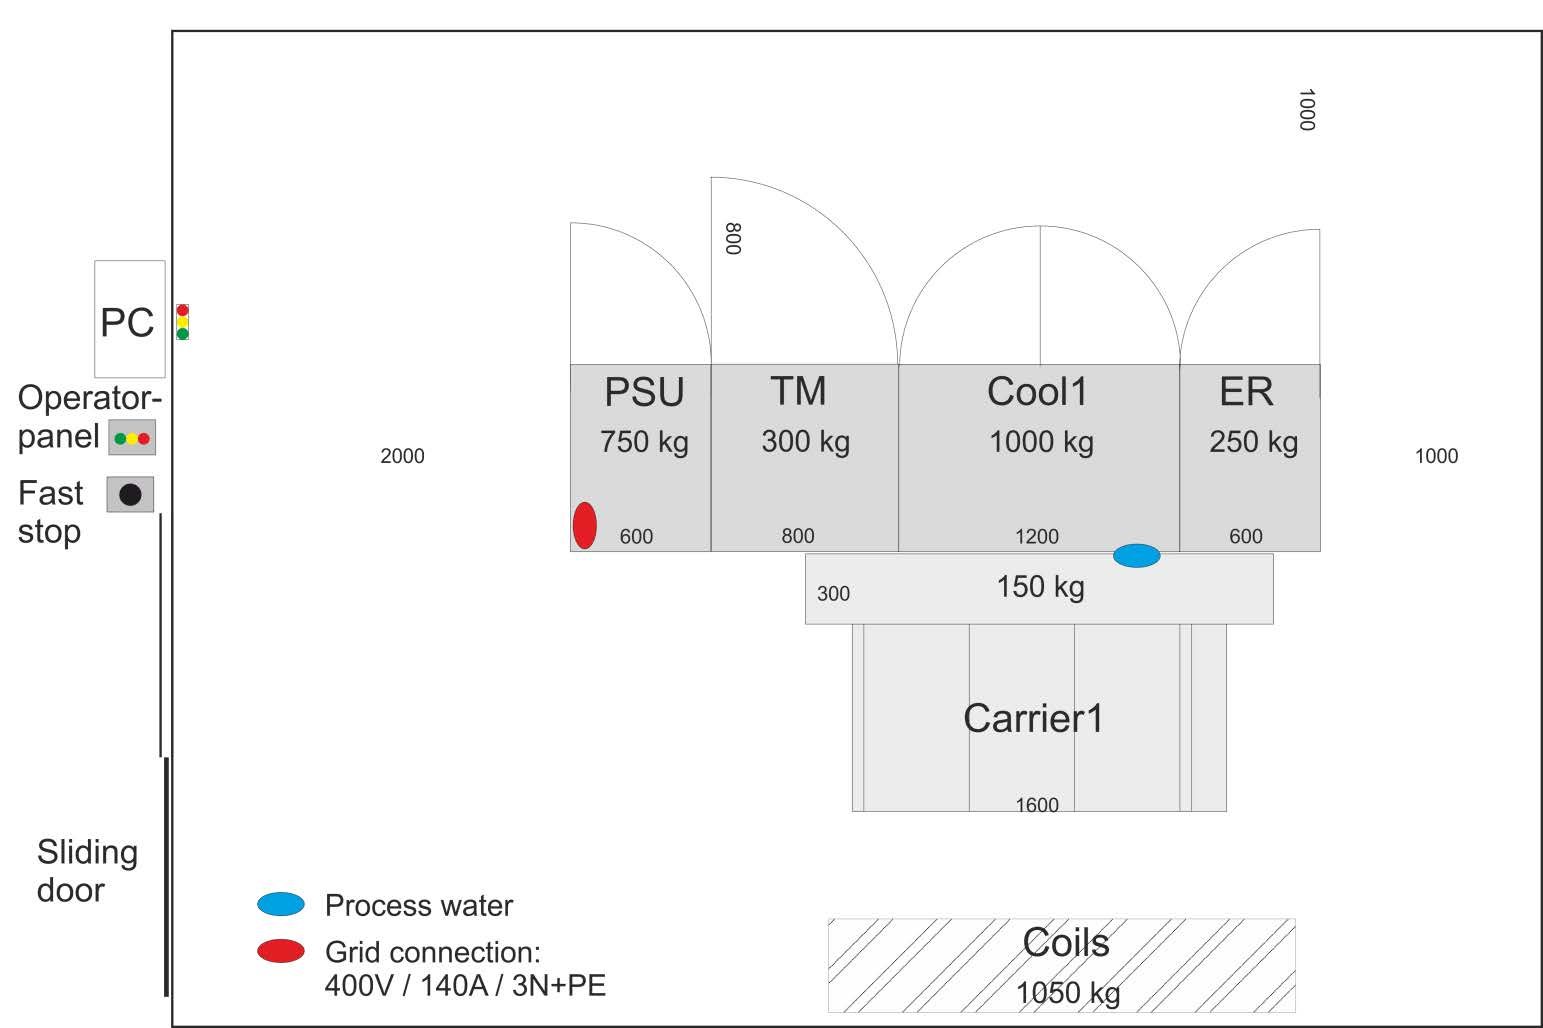
\includegraphics[width=0.8\textwidth]{Grafiken/Test Cabin}
    \caption{Aufbau des Teststandes}
    \label{fig: Aufbau des Teststandes}
    {Quelle: \cite*[7]{Main_Manuel_USTB2018}}
\end{figure}
%------------------------------------------------------------------------------------------------------
\subsubsection{Testmodule}
%------------------------------------------------------------------------------------------------------
Es gibt mehrere Testmodule, die auf dem Teststand laufen und verschiedene Funktionen der Umrichter testen.
Einige der Funktionen eines DUT können mit dem gleichen Modus eines Testmoduls überprüft werden, indem die entsprechenden Parameter ausgewählt werden.
Jeder Testablauf ist autonom und kann mehrmals ausgeführt werden, auch mit unterschiedlichen Parametern.
\\
Im Folgenden wird eine kurze Beschreibung der Funktionen der für diese Arbeit relevanten Testmodule gegeben.

Driver Consumption Test:
Der Driver Consumption Test überprüft den Stromverbrauch des Treibers im Leerlauf und während Pulssprüngen.

Pulse Test:
Der Impulstest verfügt über drei Funktionsmodi.
\begin{itemize}
    \item Im Modus \ac{FSW} kann überprüft werden, ob die Halbleiter, die sich in den \ac{DUTs} befinden, generell schalten.
    \item Im Modus \ac{OCP} kann die Überstromüberwachung weiche Kurzschlüsse überprüfen.
    Ein weicher Kurzschluss ist, wenn der Stromfluss nicht sofort und vollkommen unterbrochen wird.
    \item Im Modus \ac{DSCP} wird ein harter Kurzschluss, also ein vollständiger und sofortiger Kurzschluss, überprüft.
\end{itemize}


Power Test:
Mit diesem Test werden zwei verschiedene Funktionen getestet werden:

\begin{itemize}

    \item \ac{BIT} dient dazu, die \ac{DUTs} zyklisch zu betreiben und so reale Betriebszustände zu simulieren.
    Zudem kann mit Hilfe dieser Funktion die Kühltemperatur überprüft werden, um die korrekte Wärmeübertragung der Halbleiter sicherzustellen.
    \item Während des \ac{OTP} wird ein DUT, ähnlich wie beim \ac{BIT}, nur mit reduzierter
    Kühlung betrieben, bis die maximal zulässige Kühlkörpertemperatur erreicht ist und die Temperaturschutzschaltung auslöst.\cite*{Main_Manuel_USTB2018}

\end{itemize}

%------------------------------------------------------------------------------------------------------
\subsubsection{Testablauf}
%------------------------------------------------------------------------------------------------------
Die Schrittfolge des Testablaufes mit Montage der \ac{DUTs} ist klar festgelegt und vor jedem Durchlauf gleich.
Die Montage läuft wie folgt ab:
\begin{enumerate}

\item Die Umrichter werden auf dem Carrier befestigt. Es werden meist 3 dieser Geräte gleichzeitig getestet, Abweichungen je nach Bauform.
Die Reihenfolge der elektrischen Phasen ist bei Draufsicht des Carriers von links nach rechts U-V-W. Dies ist für das Layout des Berichtes relevant.
\item Der Kühlkreislauf wird angeschlossen, je nach Umrichtertyp Lüftungs- oder Wasserkühlung.
\item Die \ac{DUTs} werden mit den AC- und DC-Link-Kontakten verbunden, um das Gerät zu betreiben und die DC-Spannung wieder abzuleiten.
\item Das Anbringen von Signalkabeln zwischen DUT und Merkurbox. Die Merkurbox dient als Schnittstelle zwischen \ac{DUTs} und Testbench.
\item Das Montieren von VCE-Klemmen an die AC-Kontakte der \ac{DUTs}.

\end{enumerate}

Vor Beginn des Testablaufs benötigt die Test-Bench noch weitere Informationen zu den \ac{DUTs}, Testsequenzen und der Hardware-Topologie.
Diese Daten können über das Scannen von vorliegenden QR- oder Barcodes eingefügt werden.
Alternativ können diese auch über ein Eingabefenster im Teststandprogramm eingetragen werden.
Je nach Topologiekonfiguration kann auch ein zweiter Träger mit \ac{DUTs} gescannt werden,
Dies kommt bei dem Test, den das Unternehmen durchführt, nicht vor. \cite*{Main_Manuel_USTB2018}

Das eigentliche Testen mit den verschiedenen Testmodulen wird autonom durchgeführt.
Im Unternehmen läuft der Test regulär wie folgt ab:
\begin{enumerate}

\item Durchführung des Driver Consumption Testes, um die Stromversorgung der Treiberplatine auf den Umrichter zu testen.
\item Durchführung des Pulse Testes im Modus Functional-Switching, dies prüft die Umrichter.
\item Durchführung des Power Testes, in den Berichten auch XPower Test genannt.
Dieser Test simuliert die Belastung der Umrichter im Feld und überprüft,
ob sich die Werte in einem bestimmten Toleranzbereich befinden.

\end{enumerate}

Nach dem Durchlaufen eines Tests wird automatisch ein \ac{XML}-Datenfile mit den erhobenen Messdaten generiert,
die enthaltenen Messwerte und alle vorher bestimmten Einstellungen erstellt und in eine Datei eingefügt.

Bei der Demontage nach dem Testdurchlauf werden alle Schritte in umgekehrter Reihenfolge durchgeführt.
%------------------------------------------------------------------------------------------------------
\pagebreak





\subsection{Verarbeitung von XML-Daten}
\label{subsec:verarbeitung-von-xml-daten}
%------------------------------------------------------------------------------------------------------
Dieses Kapitel behandelt einige Grundlegende und für dies Arbeit relevante Aspekte von dem Dokumententype \ac{XML},
da die Messwerte bzw. die Berichte die der Testand generiert im diesem Format vorliegen.


Bei \ac{XML} handelt es sich um eine Auszeichnungssprache, also eine
formale Sprache, die verwendet werden, um die Struktur und Darstellung von Daten oder Texten zu beschreiben \cite*{Neumann2019}.
\ac{XML} wurde entwickelt, um Informationen in einem maschinenlesbaren und strukturierten Format zu speichern und zu übermitteln.
Sie wird hauptsächlich in Bereichen wie Webdiensten, Datenbanken, Konfigurationsdateien eingesetzt.
\ac{XML} ermöglicht die hierarchische Organisation von Informationen in einem strukturierten Aufbau und kann sowohl für Menschen
als auch für Maschinen interpretiert werden.\cite*{PeterBrezany2003}

Das Grundkonzept hinter \ac{XML} war, eine universelle einsetzbare und erweiterbare Sprache zu erschaffen, die von verschiedenen Systemen
unabhängig von deren grundlegenden Technologieansatz genutzt werden kann.
Hierbei ware das angestrebte Ziel Daten in einem einheitlichen Standard zwischen verschiedenen Anwendungen und Plattformen zu speichern und auszutauschen
zu kömmen.\cite*{PeterBrezany2003}
%------------------------------------------------------------------------------------------------------
\subsubsection{XML-Strukturaufbau}
%------------------------------------------------------------------------------------------------------
Eine \ac{XML}-Datei beginnt mit Prolog, der die \ac{XML}-Version und die verwendete Zeichencodierung definiert.
In Abbildung \ref{fig:XML Prolog Beispielcode} ist ein häufig genutzter Prolog dargestellt, der auch in den Teststand-Berichten genutzt wird.
Die erste Zeile des Prologs ist die sogenannte XML-Deklaration.
Die XML-Deklaration enthält häufig die Attribute sind version und encoding, jedoch nur das Attribut version ist Pflicht.
Werden auch die anderen notiert, müssen sie in der angegebenen Reihenfolge deklariert werden.
Attribut version Mit version wird die verwendete XML-Version angegeben.
Das Attribut encoding gibt die im Dokument verwendete Zeichenkodierung an, d. h. mit welcher Codierung die Datei gespeichert wird.
Fehlt die Angabe wird als Vorgabe UTF-8 (8-Bit Unicode Transformation Format) verwendet.
Neben der \ac{XML}-Deklaration können im Prolog auch noch Verarbeitungsanweisungen und Verweise auf eine \ac{DTD} deklariert werden,
dies sind jedoch optional und für diese Arbeit nicht weiter relevant.
\cite*[8,9]{Becher2022}

\begin{figure}[H]
\centering
\begin{minipage}{0.95\textwidth}
\begin{lstlisting}[language=XML]
<?xml version="1.0" encoding="UTF-8"?>
\end{lstlisting}
\end{minipage}
\caption{XML Prolog Beispielcode}
\label{fig:XML Prolog Beispielcode}
    {Quelle: eigene Darstellung}
\end{figure}


Der Hauptteil eines \ac{XML}-Dokument besteht aus einer Reihe von Elementen, die durch Tags markiert sind.
Für jedes Element gibt es ein Start- und ein EndTag, welcher das Element beginnt und beendent.
Ein Starttag kann beispeilwiese „<NamedesTags>“ so aus, dann würde der dazugehörige Endtag „</NamedesTags>“ so aussehen.
Der entscheidende Unterschied ist hierbei der Schrägstrich beim Endtag.
Der Name des Elementes wird durch den Inhalt der Keiler- und Großer-Zeichen bestimmt, bei diesem Beispiel wäre der Name „NamedesTags“.
Elemente haben einen Inhalt der aus Text, weiteren Elementen oder aus beidem bestehen kann,
wenn Elemente andere Elemente beinhalten werden Sie als Elterelemente und die enthaltenen Elemente oft Kindelemente bezeichnet.
Diese Eigenschaft der Elementente sorg dafür das XML-Datein einer hierarchischen Baumstruktur folgen.
Hierbei wird das oberste Element als Wurzelelement bezeichnet,im Englischen „root element“.\cite*[10-14]{Becher2022}


\begin{figure}[H]
\centering
\begin{minipage}{0.95\textwidth}
\begin{lstlisting}[language=XML]
<buch>
  <titel>XML-Grundlagen</titel>
  <autor>Max Mustermann</autor>
</buch>
\end{lstlisting}
\end{minipage}
\caption{XML Elemente Beispielcode}
\label{fig:XML Elemente Beispielcode}
    {Quelle: eigene Darstellung}
\end{figure}

Jedes Element kann neben Inhalt auch beliebig vielen Attributen ausgestattet sein, die zusätzliche Informationen enthalten.
Attribute werden im Start-Tag eines Elements definiert, diese bestehen immer aus eine Attributnamen und einem Wert.
Der Wert wird dabei mit Anführungszeichen deklariert, wie in Abbildung \ref{fig:XML Attribute Beispielcode} gezeigt. \cite*[10-14]{Becher2022}

\begin{figure}[H]
\centering
\begin{minipage}{0.95\textwidth}
\begin{lstlisting}[language=XML]
<buch genre="Lehrbuch">
  <titel>XML-Grundlagen</titel>
  <autor>Max Mustermann</autor>
</buch>
\end{lstlisting}
\end{minipage}
\caption{XML Attribute Beispielcode}
\label{fig:XML Attribute Beispielcode}
    {Quelle: eigene Darstellung}
\end{figure}


Kommentare werden mit den Tags „<--“ und „-->“ eingefügt und dienen der Dokumentation oder dem Hinweis auf bestimmte Teile des Codes \cite*[10-14]{Becher2022}.
Dies ist für die automatisch generierten Berichte irrelevant, jedoch für das Beschreiben der Beispiele hilfreich.
In Abbildung \ref{fig:XML Elemente Beispielcode} und Abbildung \ref{fig:XML Attribute Beispielcode} werde diese zur Beschreiben verwendet.
Kommentare werden beim Parsen des Dokuments ignoriert, parsen und Paser werden nachfolgenden Kapitel behandelt.
%------------------------------------------------------------------------------------------------------
\subsubsection{Verarbeiten von XML-Dateien}
%------------------------------------------------------------------------------------------------------
In diesem Abschnitt wird eine Zusammenfassung der grundlegenden Methoden und Techniken gegeben,
um \ac{XML}-Dateien mithilfe verschiedener Tools unabhängig von der verwendeten Programmiersprache zu verarbeiten.
Es wird beschrieben, wie man \ac{XML}-Dateien analysiert, modifiziert und überprüft, um sie für verschiedene Zwecke einsatzbereit zu machen.

Der erste Schritt beim verarbeiten einer \ac{XML}-Daten ist das Parsen.
Hierbei wird die \ac{XML}-Datei in ein Programm geladen und in ein Format umgewandelt, das das Programm interpretieren kann.
XML-Paser prüfen hierbei auch die \ac{XML}-Daten auf Korrektheit, also ob die Voralien eingehalten werden und das Dokument vollständig ist.
Dabei wird in nicht-validierte Parser und validierende Paser differenziert.
Der Unterschied besteht dadrin, dass validierte Paser neben der  korrekte Schachtelung und Bezeichnung der Strukturelemente
wie die nicht-validierten Paser auch noch auf eine Vorgabe einer Dokumenttypdefinition oder eines Schemas prüfen.\cite*[10]{Becher2022}

Paser werden verwendet um eine Applikation über eine \ac{API} eine Schnittstelle auf ein \ac{XML}-Dokument zu geben.
Bei \ac{API}s wird in diesem Bereich zwischen zwei Grundtypen unterschieden:\cite*[405]{Becher2022}

Die baumbasierten \ac{API}s lesen über den XML-Parser das XML-Dokument ein,
parst es und erzeugt ein Modell als Baum von Knoten im Arbeitsspeicher.
Auf Grunde der im XML-Dokument vorkommenden Informationseinheiten wird in verschiedene Knotentypen unterschieden.
Das generierte Modell dient der Applikation für die weitere anwendungsspezifische Verarbeitung.
Ein Beispiel für eine baumbasierte \ac{API}s ist \ac{DOM}.

\ac{DOM}ist Ein objektorientiertes Modell, das die Struktur eines XML-Dokuments abbildet.
In der Baumstruktur wird das gesamte Dokument abgebildet, indem jedes Element, Attribut und jeder Text bzw. Inhalt als Knoten gilt.
Das DOM hat den Vorteil, dass es das \ac{XML}-Dokument vollständig im Arbeitsspeicher darstellt, was das Durchsuchen und Bearbeiten des Dokuments erleichtert.
Zudem bittet es eine einfache Schnittstelle bereitstellt, um XML-Daten zu erreichen und zu verändern.
Allerdings benötigt diese Herangehensweise viel Speicherplatz,
da es das gesamte Dokument im Arbeitsspeicher ablegt, was bei großen \ac{XML}-Dokumenten ein Problem darstellen kann.\cite*[413,414]{Becher2022}


Die ereignisbasierten \ac{API}s lesen \ac{XML}-Dokument sequenziell von begin durch
ein und meldet während des Lesens jedes Ereignis durch sogenannte Callbacks an die aufrufende Applikation zurück.
Ein Ereignis ist ein Signal, das Änderungen in dem Markup-Status anzeigt.
Das Bedeutet Ereignise tritten bei Element-Tags, Zeichendaten, Kommentaren, Verarbeitungsanweisungen, sowie bei den Grenzen des Dokumentes auf.
Der Parser sendet hierbei durch die Callbacks eine Mitteilung an die aufrufende Applikation, welche Ereignisse eingetreten sind.
Das Programm, das den Parser aufgerufen hat, muss nun das Ereignis interpretieren und entsprechend reagieren.
Das \ac{XML}-Dokument wird hierbei nicht vollständig im Arbeitsspeicher gespeichert, sondern in Teilen gelesen und bearbeitet.
Deshalb eignen sich ereignisbasierte \ac{API}s besonders gut für die Verarbeitung großer \ac{XML}-Dateien, da dies für eine geringe Arbeitsspeicherbelastung sorgt.
Trotz der Effizienz hinsichtlich des Speicherverbrauchs sind ereignisbasierte \ac{API}s für die Datenmanipulation nicht sonderlich gut geeignet.
Es wird nämlich durch das Teileweise einlesen keine umfassende Dokumentstruktur wie beim aufgebaut Die baumbasierten \ac{API}s,
welches die Manipulation bzw. bearbeitung erschwert.
Ein Beispiel für eine große ereignisbasierte \ac{API} ist \ac{SAX}.
Diese \ac{API} abreitet nach dem oben beschriebenen Prinzip und wurde ursprünglich als Java-\ac{API} entwickelt, inzwischen gibt es \ac{SAX} auch für weiter Sprachen wie
z. B. C++, Perl und Python.\cite*[405]{Becher2022}

Neben diesen beide großen Beispielen gibt es auch einige kleiner Anbieter mit abgewandelten Methoden,
die jedoch in dem Umfang deutlich kleiner gehalten sind und weniger Funktionen bitten.
Ein Beispiel dafür wäre ElementTree.
ElementTree ist eine unkomplizierte und minimalistische Python-Bibliothek, die für die Bearbeitung von \ac{XML} genutzt wird.
Sie präsentiert eine Baumstruktur, die das \ac{XML}-Dokument effektiv darstellt und einfache Techniken zum Durchsuchen,
Modifizieren und Erstellen von \ac{XML}-Dokumenten bietet.\cite*{ElementTree2025}

lxml
\pagebreak

\subsection{Datenbankentwurf und Normalisierung}
\label{subsec:datenbankentwurf-und-normalisierung}
%------------------------------------------------------------------------------------------------------
Datenbanken sind strukturierte Zusammenstellungen von Daten, die elektronisch gespeichert und verwaltet werden.
Ihr Hauptziel ist es, große Datenmengen strukturiert zu speichern, den Zugriff zu optimieren und die Integrität der Daten zu gewährleisten.
Datenbanken haben im Vergleich zu anderen Dateisystemen Mechanismen, die mehreren Benutzern die parallele Nutzung ermöglichten,
sowie redundante Datenhaltung vermeiden und die effiziente Abfragen über spezielle Sprachen wie die \ac{SQL} ermöglichen.

Um den unterschiedlichen Anforderungen an Konsistenz, Flexibilität und Skalierbarkeit gerecht zu werden, ist es unerlässlich
, bei der Entwicklung moderner Informationssysteme relationale Datenbanken, dokumentenbasierte Systeme oder hybride Modelle zu verwenden.


%------------------------------------------------------------------------------------------------------
\subsubsection{Datenbankstruktur}
%------------------------------------------------------------------------------------------------------
Die Struktur der Datenbank legt fest, wie das Datenbanksystem organisiert ist und wie die Datenelemente angeordnet sind.
Das Grundprinzip relationaler Datenbanken sind im Grunde Tabellen und die Beziehungen zwischen diesen.
Die Hauptbestandteile sind:

\begin{itemize}
\item Tabellen – das grundlegende Element, welches Daten in Zeilen (Tupeln) und Spalten (Attributen) strukturiert.
\item Ein Datensatz in einer Tabelle wird durch Primärschlüssel (Primary Keys) eindeutig identifiziert.
\item Schlüssel aus anderen Tabellen (Foreign Keys)  Tabellenverknüpfung, um die referenzielle Integrität zu gewährleisten.
\item Indizes: Datenstrukturen, die das Beschleunigen von Abfragen ermöglichen.
\item Views: sie sind virtuelle Tabellen und beruhen auf den Ergebnissen von Abfragen.
\item Constraints: Vorgaben zur Gewährleistung der Datenintegrität (z.B. Wertebereiche, Pflichtfelder oder Dopplungen).
\end{itemize}
%------------------------------------------------------------------------------------------------------
\subsubsection{Datenintegrität und Normalisierung}
%------------------------------------------------------------------------------------------------------
Ein methodischer Ansatz zur Reduzierung von Redundanzen und Anomalien ist die Normalisierung.
Der Prozess erfolgt schrittweise durch die Normalformen, die durch Indizes  (1NF, 2NF, 3NF, BCNF) definiert sind.
Alle Normalformen haben spezifische Arten von Datenanomalien zum Ziel:

\begin{itemize}

\item 1. Normalform (1NF): Beseitigung mehrfacher Werte innerhalb einer Zelle;  atomare Attribute.
\item 2. Normalform (2NF): Beseitigung partieller Abhängigkeiten.
\item 3. Normalform (3NF): Beseitigung transitiver Abhängigkeiten.

\end{itemize}

Die Gewährleistung, dass Daten korrekt, konsistent und vollständig sind,
fällt unter das Konzept der Datenintegrität.
Sie wird erzielt durch:

\begin{itemize}
\item
Entity-Integrität (eindeutige Primärschlüssel).
\item
Referentielle Integrität (gültige Fremdschlüsselverweise).

\item Domänenintegrität (gültige Wertebereiche und Datentypen).
\item Entity-Integrität (eindeutige Primärschlüssel).
\item Referentielle Integrität (gültige Fremdschlüsselverweise).
\item Integrität der Domäne (gültige Wertebereiche und Datentypen).

\end{itemize}

%------------------------------------------------------------------------------------------------------
\subsubsection{Vorgehen zur Erstellung der Datenbank}
%------------------------------------------------------------------------------------------------------
Bei der Erstellung einer Datenbank sollte nach folgendem Schema vorgegangen werden.
Bei diesem Schema gilt es, sowohl technische als auch konzeptionelle Aspekte zu berücksichtigen:

\begin{enumerate}

\item
Anforderungsanalyse

Zuerst wird im Hinblick auf das Geschäftsumfeld bestimmt, welchen konkreten Zweck die Datenbank erfüllen soll.
Hierbei ist die Zweckbestimmung  entscheidend, da sie festlegt, welche Daten als relevant gelten.
Der Konzeptvorschlag, der das Projektziel definiert und die Vorgehensweise umreißt, ist das Ergebnis.
\begin{itemize}

\item
Festlegung der fachlichen und technischen Voraussetzungen.
\item
Bestimmung der relevanten Datenquellen und -formate.
\item
Definition von Integritäts- und Sicherheitsanforderungen.

\end{itemize}

\item
Konzeptionelles Datenmodell

Es soll das geschäftliche Umfeld betrachtet werden.
Die bestehende Objekte (z.B. Reports mit Materialnummer, Datum, Version), deren Attribute sowie die Beziehungen und Einschränkungen zwischen diesen Objekten.
Das Entity-Relationship-Modell (ERM) nach Chen oder das PrecisedERM (PERM) werden häufig zur Modellierung verwendet.
Der konzeptionelle Entwurf ist die Grundlage für die nächste Phase und dient als Diskussionsgrundlage.
\begin{itemize}

\item Die Entwicklung eines Entity-Relationship-Modells (ERM), das die reale Welt in Entitäten, Attribute und Beziehungen abbildet.
\item Die Einbeziehung von Kardinalitäten (1:1, 1:n, n:m).

\end{itemize}

\item
Logisches Datenmodell

Der konzeptionelle Entwurf wird in einen logischen Entwurf umgewandelt, der die fachlichen Konzepte in ein datenbanktechnisches Format überführt.
In der Regel kommt das Relationenmodell zum Einsatz, welches die Daten in Form von Tabellen organisiert.
Transformationsregeln garantieren, dass Beziehungen und Integritätsbedingungen richtig umgesetzt werden.
\begin{itemize}

\item Transformation des konzeptionellen Modells in ein relationales Schema.
\item Festlegung von Tabellen, Spalten (Attribute), Primärschlüsseln und Fremdschlüsseln.
\item Definition von Datentypen und Zellenkofigurationen (z.B. NOT NULL, UNIQUE, CHECK).
\end{itemize}

\item
Physisches Datenmodell

Eine physische Datenbankstruktur wird durch \as{SQL} erstellt, basierend auf dem logischen Entwurf.
Die konkrete Festlegung von Tabellen, Indizes, Constraints usw. erfolgt dabei durch  Das System,
das wir implementiert haben, wird immer wieder getestet und zusammen mit den Nutzerinnen auf fachliche Richtigkeit überprüft.
\begin{itemize}

\item Realisierung des logischen Modells in einer spezifischen Datenbankmanagementsoftware (z.B. MySQL, Mariadb oder Microsoft SQL Server).er).
\item Die Verbesserung der Speicherstrukturen, der Indexierung und der Partitionierung.

\end{itemize}

\item
Implementierung und Prüfung

Nach der erfolgreichen Umsetzung wird das System vom Kunden gemäß einem vorher festgelegten Abnahmeplan freigegeben.
Ein Wartungsplan kümmert sich anschließend um die Betreuung, schult die Endbenutzer und überwacht die IT-Umgebung kontinuierlich.
\begin{itemize}

\item Den Aufbau der Tabellen und Relationen entsprechend dem Datenbankschema.

\item Die Testdaten implementieren.

\item Die Kontrolle der Funktionalität und Leistung.

\end{itemize}

\end{enumerate}

\pagebreak


\subsection{Grundlagen der Datenvisualisierung}
\label{subsec:grundlagen-der-datenvisualisierung}

\subsubsection{Begriff und Zielsetzung}

Unter Datenvisualisierung wird die visuelle Aufbereitung von Daten verstanden, um Muster, Trends, Zusammenhänge
oder Anomalien erkennbar zu machen.
Sie stellt ein zentrales Hilfsmittel dar, um komplexe Informationen effizient zu kommunizieren und kognitive
Verarbeitungsprozesse zu unterstützen[Shneiderman, 1996].
Durch die grafische Darstellung wird es dem Betrachter ermöglicht, große Datenmengen intuitiv zu erfassen,
ohne ausschließlich auf numerische oder textuelle Formen angewiesen zu sein.
Die Zielsetzung der Datenvisualisierung umfasst in der Regel drei Kernaspekte[Ware, 2021]:

\begin{enumerate}

\item
Exploration: Unterstützung bei der Entdeckung neuer Zusammenhänge und Hypothesen.
\item
Analyse: Erleichterung der detaillierten Untersuchung von Strukturen und Abhängigkeiten.
\item
Kommunikation: Vermittlung von Ergebnissen an unterschiedliche Zielgruppen.

\end{enumerate}

\subsubsection{Theoretische Grundlagen}

Die Grundlage wirksamer Datenvisualisierung liegt in der menschlichen Wahrnehmungspsychologie.
Insbesondere die Gestaltungsgesetze (z.B. Gesetz der Nähe, Ähnlichkeit und Kontinuität) spielen eine zentrale Rolle,
da sie bestimmen, wie Informationen visuell gruppiert und interpretiert werden[Wertheimer, 1923].

Zusätzlich beschreibt die Theorie der \textit{kognitiven Belastung} (Cognitive Load Theory),
dass Darstellungen so gestaltet werden sollten, dass sie die Arbeitsgedächtniskapazität nicht überlasten[Sweller, 1988].


Ein weiterer theoretischer Rahmen ist Shneidermans Visual Information-Seeking Mantra:



„Overview first, zoom and filter, then details-on-demand.“

Dieses Prinzip betont die Notwendigkeit einer schrittweisen Annäherung an Daten, um vom Gesamtüberblick bis hin zu
spezifischen Details zu gelangen.


\subsubsection{Formen der Datenvisualisierung}

Datenvisualisierungen lassen sich in verschiedene Kategorien einteilen[Few, 2012]:

\begin{itemize}

\item
Explorative Visualisierung: Interaktive Darstellungen, die zur Untersuchung und Hypothesengenerierung dienen.
\item
Explikative Visualisierung: Fokussierte, oft statische Darstellungen, die Ergebnisse gezielt kommunizieren.
\item
Interaktive Dashboards: Kombination mehrerer Visualisierungstypen, häufig für Monitoring und Entscheidungsunterstützung.

\end{itemize}

Je nach Datentyp und Analyseziel kommen unterschiedliche Diagrammformen und Techniken zum Einsatz:

\begin{itemize}

\item
Zeitreihen: Liniendiagramme, Flächendiagramme
\item
Kategorische Daten: Balken- und Säulendiagramme
\item
Zusammenhänge: Streudiagramme, Blasendiagramme
\item
Verteilungen: Histogramme, Boxplots
\item
Hierarchien und Netzwerke: Baumdiagramme, Graphvisualisierungen

\end{itemize}

\subsubsection{Qualitätskriterien}

Eine gute Datenvisualisierung erfüllt folgende Kriterien[Tufte, 2001]:


\begin{itemize}

\item
Klarheit: Vermeidung unnötiger grafischer Elemente („Chartjunk“)
\item
Genauigkeit: Wahrheitsgetreue Darstellung ohne Verzerrung von Skalen oder Proportionen
\item
Effizienz: Schnelle Erfassbarkeit der relevanten Information
\item
Ästhetik: Ansprechende Gestaltung zur Förderung der Akzeptanz
\item
Barrierefreiheit: Berücksichtigung farbsehschwacher Nutzer durch geeignete Farbpaletten

\end{itemize}

\subsubsection{Technologische Aspekte}

Mit dem Fortschritt moderner IT-Systeme haben sich leistungsfähige Werkzeuge und Bibliotheken für die
Datenvisualisierung etabliert.
Beispiele sind Matplotlib und Plotly im Python-Umfeld, D3.js im Webbereich.

In Webapplikationen ermöglichen interaktive Bibliotheken eine nahtlose Einbettung in Benutzeroberflächen,
wodurch sowohl explorative als auch explikative Ziele unterstützt werden.

\subsubsection{Graphen erstellung mit JS}


\subsection*{Chart.js}

Eine einfache und beliebte Bibliothek für Standarddiagramme wie Balken, Linien oder Kreisdiagramme. Schnell eingebunden, gute Standardoptik, ideal für kleinere Projekte oder schnelle Visualisierungen.



\subsection*{D3.js}

Eine sehr mächtige Low-Level-Bibliothek, die mit SVG, Canvas und HTML arbeitet. Extrem flexibel für individuelle und interaktive Visualisierungen, aber mit einer steilen Lernkurve.



\subsection*{Plotly.js}

Bietet viele interaktive Diagramme (Zoom, Hover, Export als PNG). Unterstützt auch 3D- und wissenschaftliche Charts. Gut geeignet für Dashboards und Datenanalyse.



\subsection*{ECharts (Apache ECharts)}

Eine leistungsstarke Open-Source-Bibliothek von Apache. Unterstützt viele Diagrammtypen (inkl. Heatmaps, Maps, Candlesticks) mit Animationen und Interaktivität. Besonders beliebt für komplexe Enterprise-Web-Apps.



\subsection*{Highcharts}

Eine professionelle, kommerzielle Lösung (kostenlos für private Nutzung). Sehr einfach konfigurierbar, liefert Business-taugliche Diagramme mit vielen Optionen. Oft in Unternehmen eingesetzt.



\subsection*{vis.js}

Spezialisiert auf Netzwerk- und Zeitachsenvisualisierungen. Eignet sich besonders für Knoten-Graphen, Beziehungen oder Prozessdiagramme mit Interaktivität.



\subsection*{Recharts}

Eine React-spezifische Bibliothek, die auf D3.js basiert. Bietet eine einfache Komponenten-API für gängige Diagramme. Ideal, wenn deine Web-App mit React entwickelt ist.



\pagebreak



\section{Anforderungen an modulare Softwareentwicklung (nach ISO/IEC 9126)}
\label{sec:anforderungen-an-modulare-softwareentwicklung-(nach-iso/iec-9126)}

Die Norm \textbf{ISO/IEC 9126} beschreibt ein Qualitätsmodell für Softwareprodukte, das mehrere Haupt- und Untermerkmale definiert.
Diese Merkmale lassen sich auf die modulare Softwareentwicklung übertragen, da sie zentrale Eigenschaften wie Wartbarkeit, Erweiterbarkeit und Austauschbarkeit quantifizierbar machen.
Eine modulare Architektur erfüllt diese Qualitätsziele durch klar definierte Schnittstellen, lose Kopplung und eine hohe Kohäsion der Module.\cite{ISOIEC9126-1991}

\begin{itemize}
    \item \textbf{Funktionalität:}
    Jedes Modul soll die vorgesehenen Aufgaben korrekt und zweckmäßig ausführen.
    Eine hohe Funktionalität setzt voraus, dass Module die geforderten Spezifikationen erfüllen, interoperabel mit anderen Komponenten sind und relevante Standards einhalten.
    \emph{Untermerkmale: Eignung, Korrektheit, Interoperabilität, Konformität, Sicherheit.}

    \item \textbf{Zuverlässigkeit:}
    Module sollen auch unter unerwarteten Bedingungen stabil arbeiten und definierte Wiederherstellungsmechanismen besitzen.
    Eine hohe Zuverlässigkeit gewährleistet, dass Fehlfunktionen lokal begrenzt bleiben und das Gesamtsystem funktionsfähig bleibt.
    \emph{Untermerkmale: Reife, Fehlertoleranz, Wiederherstellbarkeit.}

    \item \textbf{Benutzbarkeit:}
    Module und Schnittstellen sollen verständlich, erlernbar und bedienbar sein.
    Diese Anforderung gilt sowohl für Benutzerschnittstellen als auch für APIs, um eine konsistente Integration und Nutzung zu ermöglichen.
    \emph{Untermerkmale: Verständlichkeit, Erlernbarkeit, Bedienbarkeit.}

    \item \textbf{Effizienz:}
    Module sollen vorhandene Ressourcen optimal nutzen und geforderte Leistungswerte einhalten.
    Eine effiziente Implementierung trägt zu einem stabilen Laufzeitverhalten und einer guten Skalierbarkeit des Gesamtsystems bei.
    \emph{Untermerkmale: Zeitverhalten, Ressourcenverhalten.}

    \item \textbf{Wartbarkeit:}
    Module sollen leicht analysierbar, anpassbar und testbar sein.
    Änderungen müssen möglichst lokal vorgenommen werden können, ohne unbeabsichtigte Auswirkungen auf andere Systemkomponenten zu verursachen.
    \emph{Untermerkmale: Analysierbarkeit, Änderbarkeit, Stabilität, Testbarkeit.}

    \item \textbf{Portabilität:}
    Module sollen an unterschiedliche Zielumgebungen anpassbar und bei gleichbleibender Schnittstelle austauschbar sein.
    Dadurch wird die Wiederverwendung und langfristige Nutzbarkeit der Software verbessert.
    \emph{Untermerkmale: Anpassbarkeit, Installierbarkeit, Konformität, Austauschbarkeit.}
\end{itemize}

Die Berücksichtigung dieser Qualitätsmerkmale bei der Entwicklung modularer Systeme stellt sicher, dass Software langfristig wartbar, erweiterbar und zuverlässig bleibt.
Das Qualitätsmodell der ISO/IEC 9126 bietet damit eine strukturierte Grundlage zur Bewertung und Verbesserung der architektonischen Qualität modularer Anwendungen. \cite{ISOIEC9126-1991}


\pagebreak